% flashcards-title: Model and evidence loop
% flashcards-desc: Four nodes labeled Model, Prediction, Measurement, and Compare form a clockwise loop. A dashed return arrow connects comparison back to the model.
\documentclass[border=5mm]{standalone}
\def\pgfsysdriver{pgfsys-dvisvgm.def}
\usepackage{tikz}
\usetikzlibrary{arrows.meta,calc,patterns.meta,positioning}
\renewcommand{\familydefault}{\sfdefault}

\definecolor{fcInk}{HTML}{1C1C1E}
\definecolor{fcMuted}{HTML}{68686D}
\definecolor{fcGuide}{HTML}{C9C9CE}
\definecolor{fcGold}{HTML}{D7A313}
\definecolor{fcGoldSoft}{HTML}{F8E8AE}

\tikzset{
  fc canvas/.style={fill=white, rounded corners=2.5mm},
  fc vector/.style={
    draw=fcGold,
    line width=1.35mm,
    line cap=round,
    -{Stealth[length=4.1mm,width=3.25mm]}
  },
  fc vector secondary/.style={
    draw=fcInk,
    line width=1.15mm,
    line cap=round,
    dash pattern=on 4.1mm off 2.6mm,
    -{Stealth[length=3.9mm,width=3.1mm]}
  },
  fc resultant/.style={
    draw=fcMuted,
    line width=1.55mm,
    line cap=round,
    -{Stealth[length=4.6mm,width=3.6mm]}
  },
  fc axis/.style={
    draw=fcInk,
    line width=.72mm,
    -{Stealth[length=3.1mm,width=2.5mm]}
  },
  fc guide/.style={
    draw=fcMuted,
    line width=.55mm,
    dash pattern=on 2.3mm off 1.8mm
  },
  fc construction/.style={draw=fcGuide, line width=.32mm},
  fc endpoint/.style={circle, fill=fcInk, inner sep=1.45mm},
  fc label/.style={font=\bfseries\large, text=fcInk},
  fc small label/.style={font=\small, text=fcMuted},
  fc caption/.style={font=\bfseries\small, text=fcMuted}
}

\begin{document}
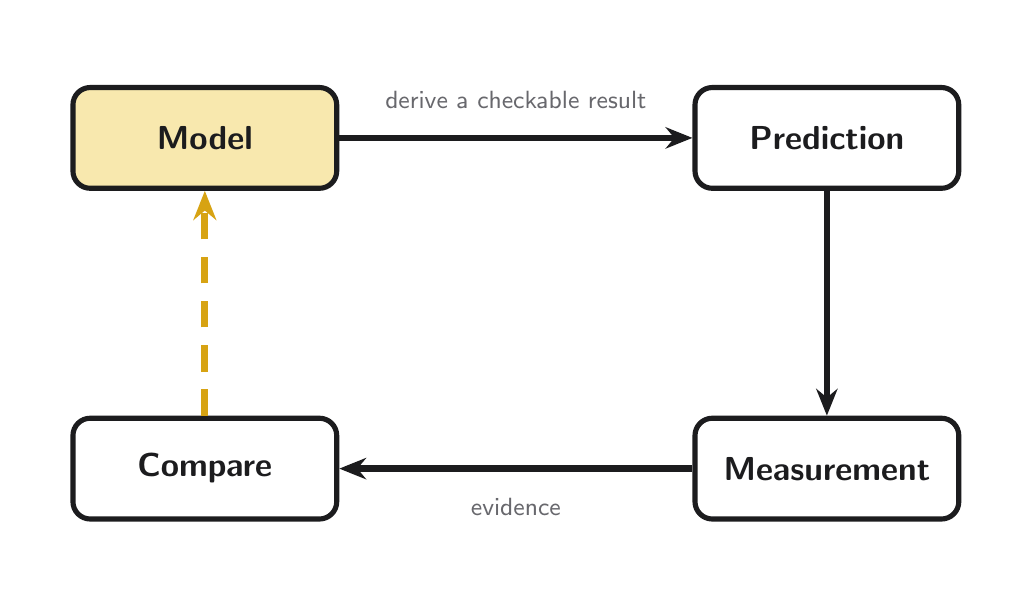
\begin{tikzpicture}[x=1cm,y=1cm]
  \path[fc canvas] (-.45,-.45) rectangle (11.95,6.65);
  \tikzset{
    fc process/.style={
      draw=fcInk,
      fill=white,
      line width=.65mm,
      rounded corners=2.2mm,
      minimum width=3.35cm,
      minimum height=1.28cm,
      font=\bfseries\large,
      text=fcInk,
      align=center
    },
    fc process accent/.style={fc process, fill=fcGoldSoft},
    fc flow/.style={
      draw=fcInk,
      line width=.82mm,
      -{Stealth[length=3.4mm,width=2.7mm]}
    },
    fc return/.style={
      draw=fcGold,
      line width=.92mm,
      dash pattern=on 3.4mm off 2.2mm,
      -{Stealth[length=3.7mm,width=2.9mm]}
    }
  }

  \node[fc process accent] (model) at (1.8,5.25) {Model};
  \node[fc process] (prediction) at (9.7,5.25) {Prediction};
  \node[fc process] (measurement) at (9.7,1.05) {Measurement};
  \node[fc process] (compare) at (1.8,1.05) {Compare};

  \draw[fc flow] (model.east) -- (prediction.west)
    node[midway, above=2.2mm, fc small label] {derive a checkable result};
  \draw[fc flow] (prediction.south) -- (measurement.north);
  \draw[fc flow] (measurement.west) -- (compare.east)
    node[midway, below=2.2mm, fc small label] {evidence};
  \draw[fc return] (compare.north) -- (model.south);
\end{tikzpicture}
\end{document}
